%----------------------------------------------------------------------------------------
%	PACKAGES AND THEMES
%----------------------------------------------------------------------------------------
\documentclass[aspectratio=169, t]{beamer}

\mode<presentation> {
\usetheme{Madrid}
\setbeamertemplate{navigation symbols}{}
}

\usepackage{graphicx}
\usepackage{booktabs}
\usepackage{pdfpages}

%----------------------------------------------------------------------------------------
%	TITLE PAGE0
%----------------------------------------------------------------------------------------
\title[Designing a Badge Add-on in KiCad]{Designing a Badge Add-on in KiCad}

\author{Josh Johnson}
\date{BSides Canberra 2023}

\begin{document}
\begin{frame}
\titlepage
\end{frame}

%----------------------------------------------------------------------------------------
%	PRESENTATION SLIDES
%----------------------------------------------------------------------------------------
\begin{frame}
\frametitle{Overview}
\begin{columns}
	\column{.54\textwidth}
		\begin{itemize}
			\item Install KiCad: kicad.org
			\item Open the workshop instructions: joshajohnson.com/bsidescbr23-workshop/
			\item Download the KiCad library linked in the workshop instructions
			\item Files also available on USB drives
			\item Use a mouse
			\item Ask and any all questions!
		\end{itemize}
	
	\column{0.45\textwidth}
		\begin{figure}
			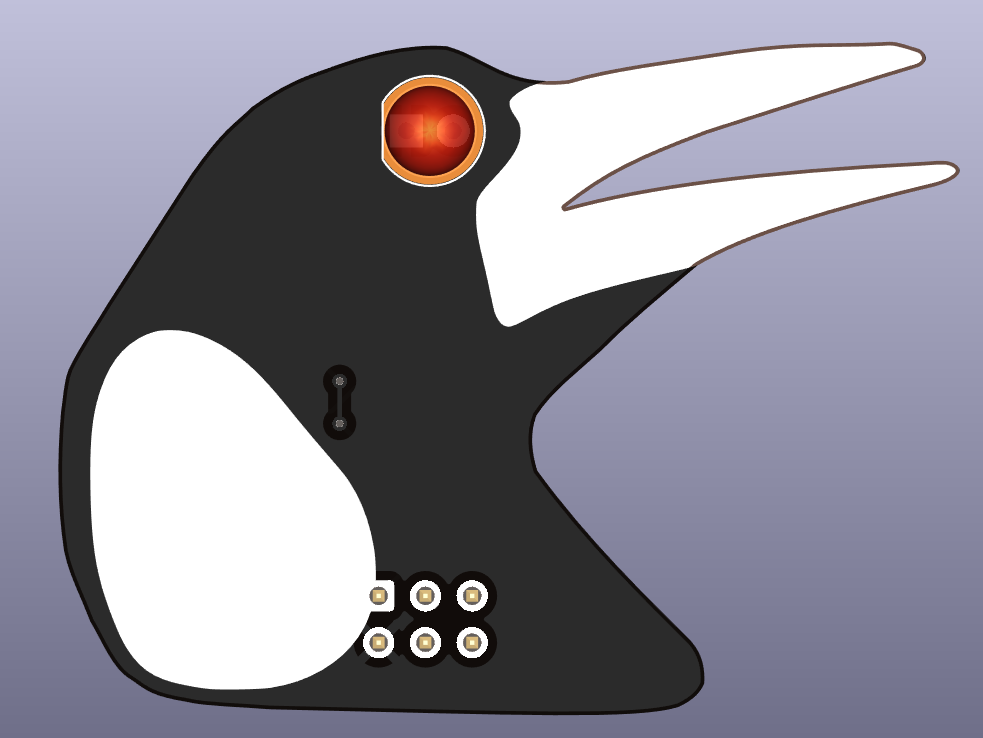
\includegraphics[width=1.0\linewidth]{images/magpie_render.png}
		\end{figure}
\end{columns}
\end{frame}

%----------------------------------------------------------------------------------------
\begin{frame}
	\frametitle{Presenters}
	\begin{columns}
		\column{.54\textwidth}
		Josh
			\begin{itemize}
				\item Electronics Engineer
				\item Day job: automotive, telecommunications, aerospace
				\item Arvo job: LEDs, keyboards, RF, FPGAs, workshops, FIRST Robotics
				\item Fun: Mountain biking, running
			\end{itemize}
		\vspace{1em}
		Peter
		\begin{itemize}
			\item Security Researcher
			\item Hardware and Firmware for bPod
			\item Repurposing old iPods, iMacs
		\end{itemize}
		
		\column{0.45\textwidth}
		\vspace{-8mm}
			\begin{figure}
				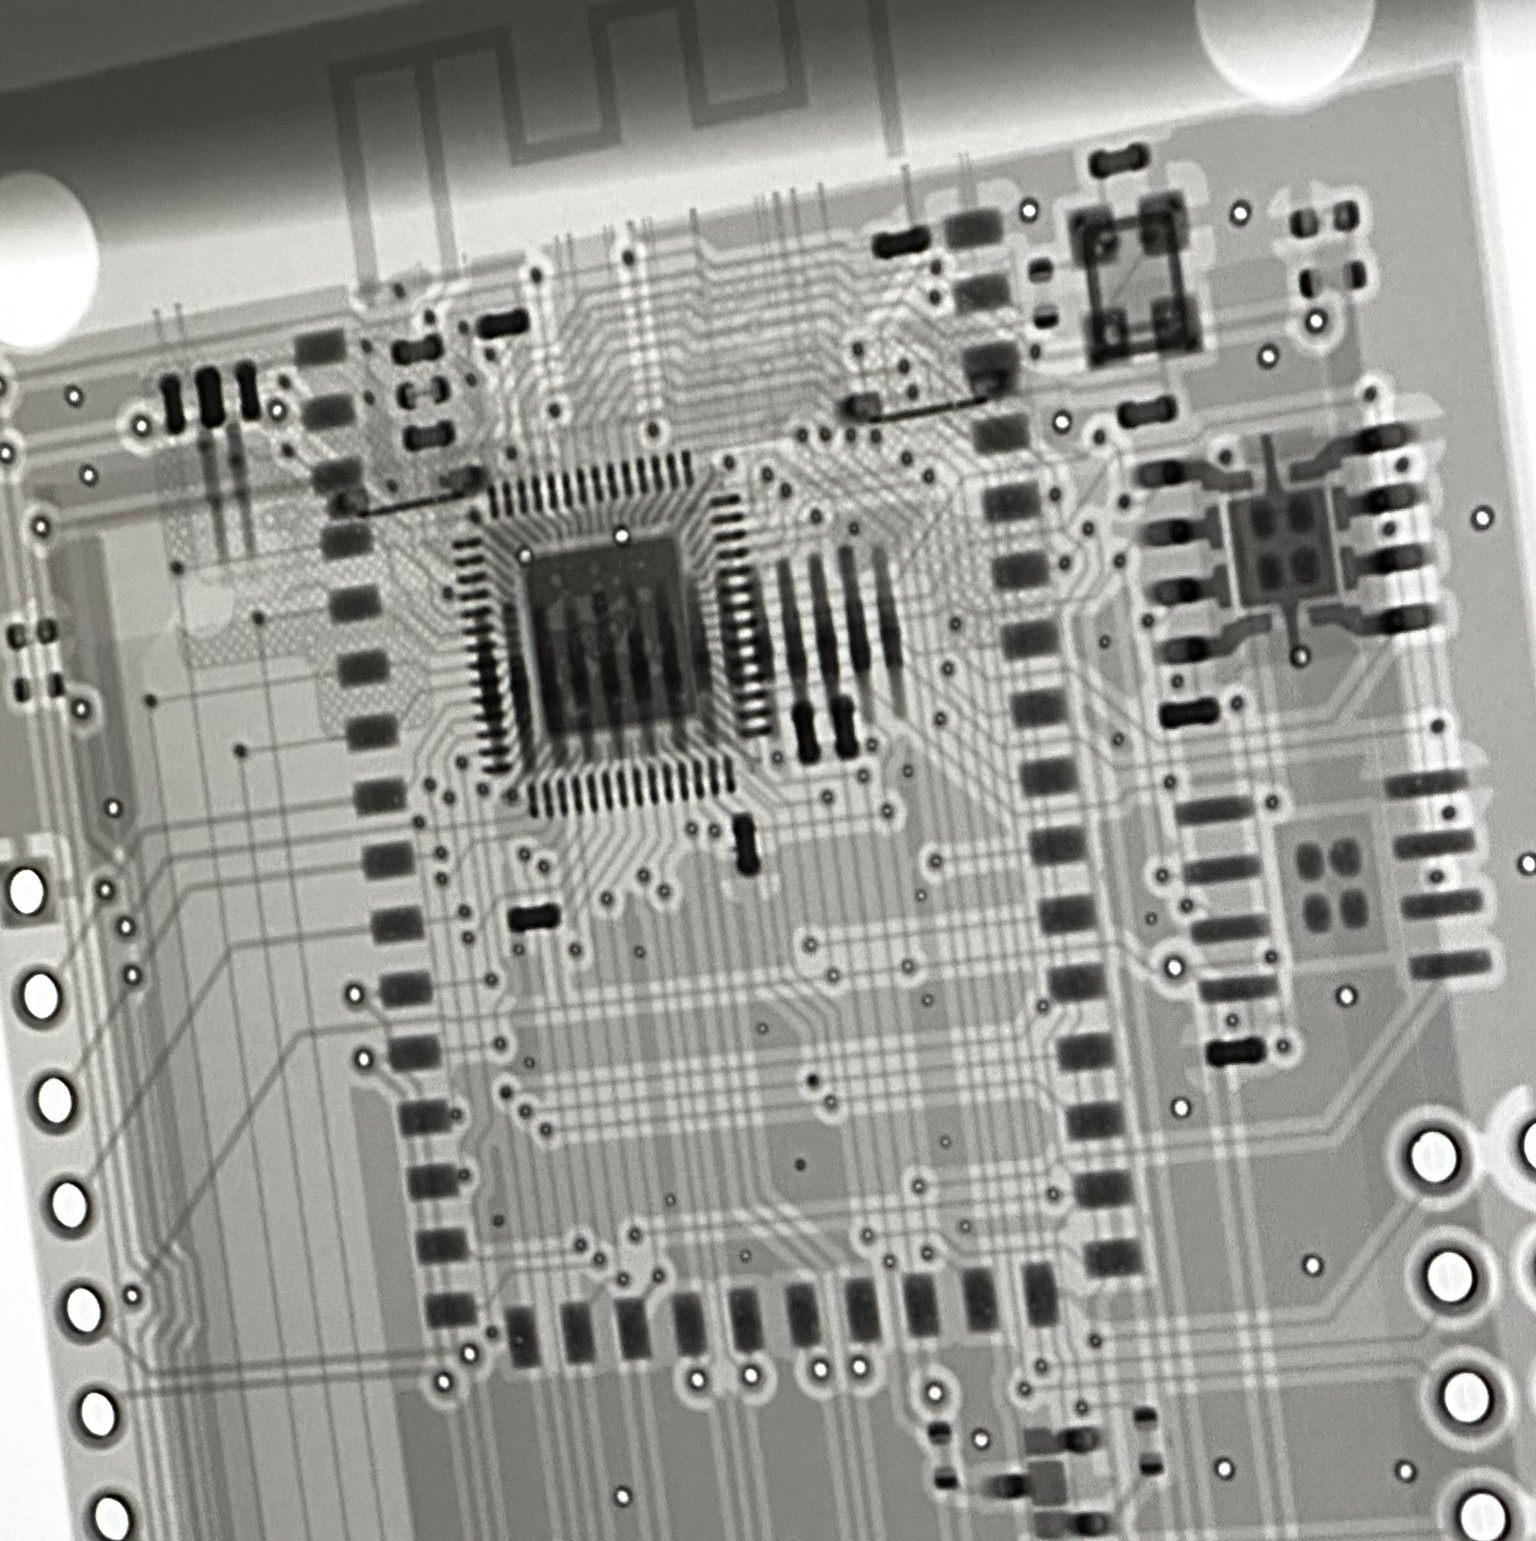
\includegraphics[width=0.9\linewidth]{images/bpod_xray.jpeg}
			\end{figure}
			\centering
			\text{Image: Infosect}
	\end{columns}
	\end{frame}

%----------------------------------------------------------------------------------------
\begin{frame}
	\frametitle{Schedule}
	\begin{columns}
		\vspace{-8mm}
		\column{.54\textwidth}
			\begin{itemize}
				\item Introduction
				\item Schematic Capture
				\item PCB Layout
				\item Assembly
			\end{itemize}

		\vspace{1em}

		Each section consists of:
		\begin{itemize}
			\item One slide summary
			\item Demo of the required steps
			\item Time to do it yourself
		\end{itemize}
		
		\column{0.45\textwidth}
			\begin{figure}
				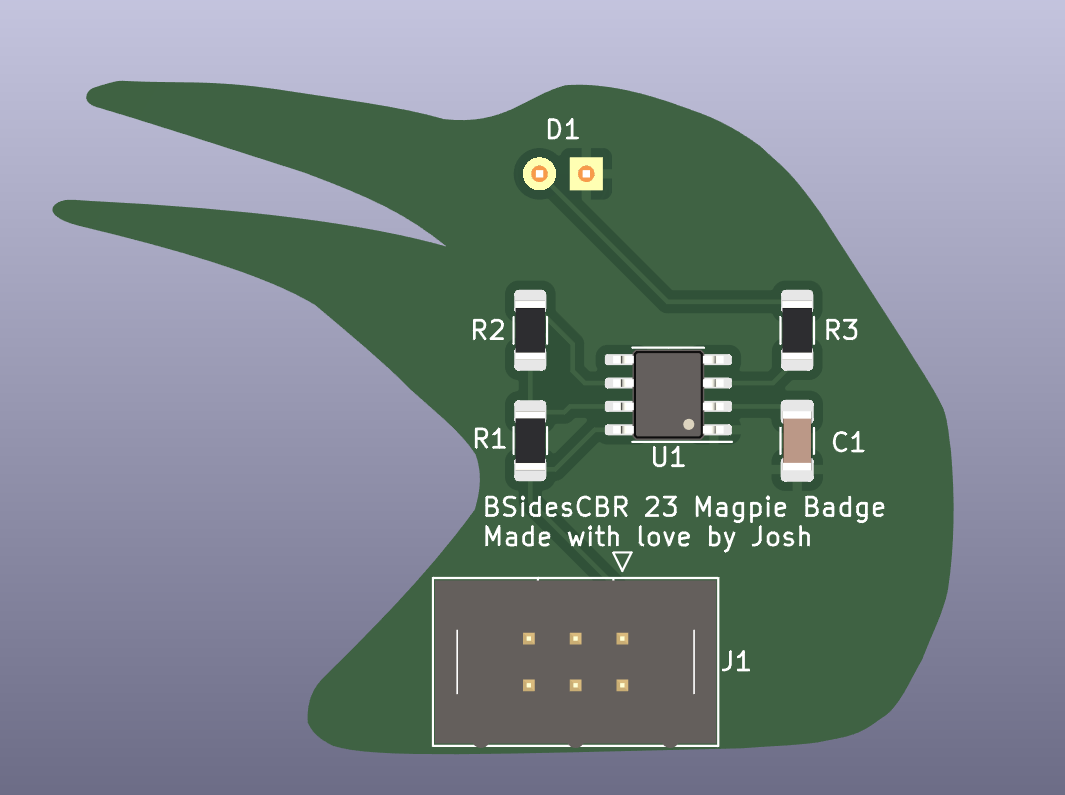
\includegraphics[width=1.0\linewidth]{images/cleanup_silk.png}
			\end{figure}
	\end{columns}
	\end{frame}

%----------------------------------------------------------------------------------------
\begin{frame}
	\frametitle{Scope}	
	\begin{columns}
		\column{.6\textwidth}
		In scope
		\begin{itemize}
			\item Schematic capture in KiCad
			\item PCB layout in KiCad
			\item Exporting Gerbers from KiCad
			\item Prototype assembly
		\end{itemize}

		Out of scope
		\begin{itemize}
			\item Circuit design
			\item PCB design best practices
			\item Generating magpie artwork
			\item Using other CAD tools
			\item Mechanical / enclosure design
		\end{itemize}
		
		Happy to chat about anything after the workshop!
		\column{0.4\textwidth}
		\vspace{-8mm}
		\begin{figure}
			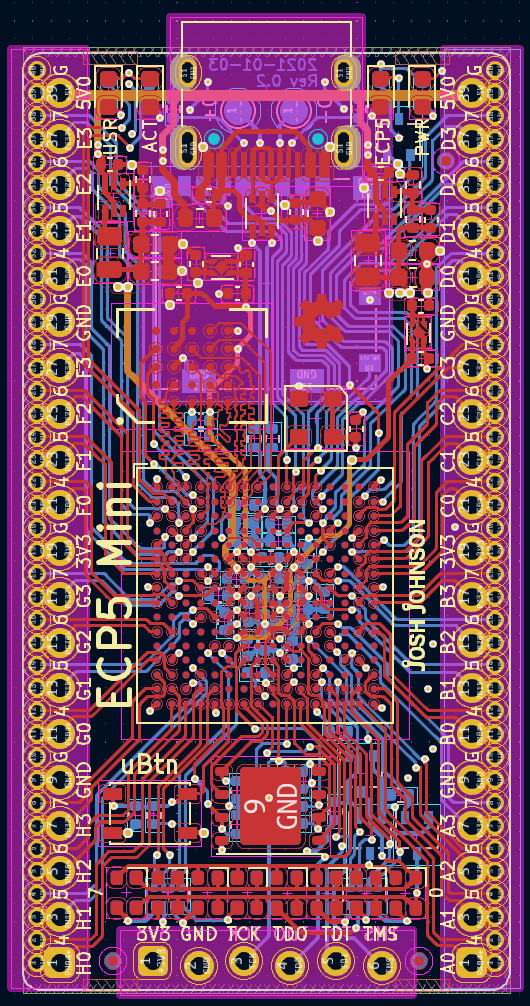
\includegraphics[width=0.6\linewidth]{images/ecp5_mini.png}
		\end{figure}

	\end{columns}


\end{frame}

%----------------------------------------------------------------------------------------
\begin{frame}
\frametitle{Schematic Capture}
\begin{columns}
	\column{.6\textwidth}
	What: Abstract representation of circuit / components.\\
	Why: Communicates purpose and documents design.\\
	How:
	\begin{itemize}
		\item Symbol creation
		\item Symbol placement
		\item Connect everything with wires
		\item Add notes to your design
		\item Run electrical rules checks (ERC)
		\item Footprint association (may be done in symbol placement)
		\item Bill of Materials (BOM) generation
	\end{itemize}
	
	\column{0.39\textwidth}
	\vspace{-8mm}
	\begin{figure}
		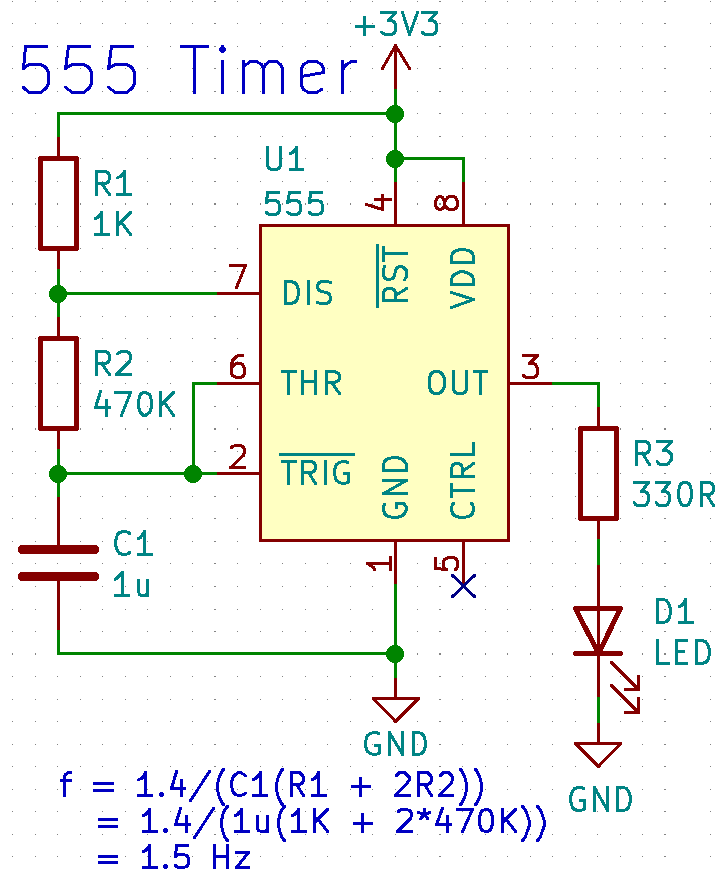
\includegraphics[width=\linewidth]{images/555-schematic-snip.png}
	\end{figure}
\end{columns}
\end{frame}

%----------------------------------------------------------------------------------------
\begin{frame}
	\frametitle{PCB Layers}
	\vspace{-2mm}
	\begin{figure}
			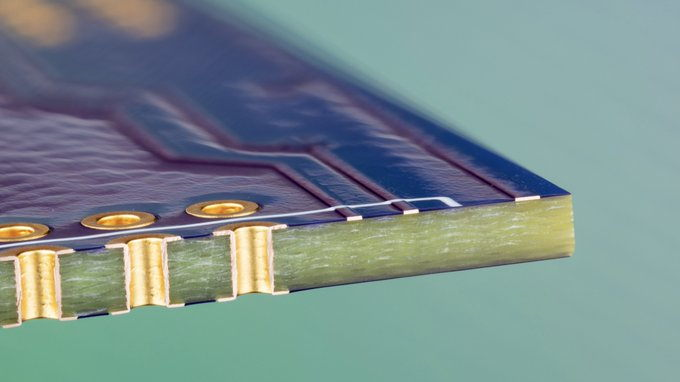
\includegraphics[width=11cm]{images/esml_2_layer.jpeg}
	\end{figure}
	\centering
	\text{Image: EMSL}
\end{frame}

%----------------------------------------------------------------------------------------
\begin{frame}
\frametitle{PCB Layout}
\begin{columns}
	\column{.6\textwidth}
	What: Physical representation of circuit / components.\\
	Why: Ensures electrical and mechanical function.\\
	How:
	\begin{itemize}
		\item Configure design rules per manufacturer guidelines
		\item Draw board outline
		\item Place connectors and mounting holes
		\item Place electronic components
		\item Route critical nets, power, then everything else
		\item Run design rule checks (DRC)
		\item Add decorative features
		\item Review in 3D viewer / check mechanical fit
		\item Export Gerbers
	\end{itemize}
	
	\column{0.39\textwidth}
	\vspace{-7mm}
	\begin{figure}
		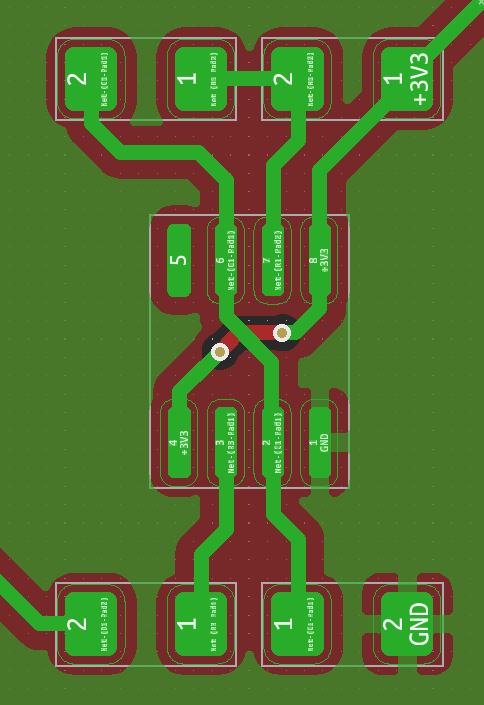
\includegraphics[width=0.8\linewidth]{images/555-layout.png}
	\end{figure}
\end{columns}
\end{frame}

%----------------------------------------------------------------------------------------
\begin{frame}
\frametitle{Prototype Assembly}
	\begin{itemize}
		\item Solder surface mount
		\item Solder through hole
		\item Inspect for defects
		\item Smoke test
	\end{itemize}	

\begin{figure}
	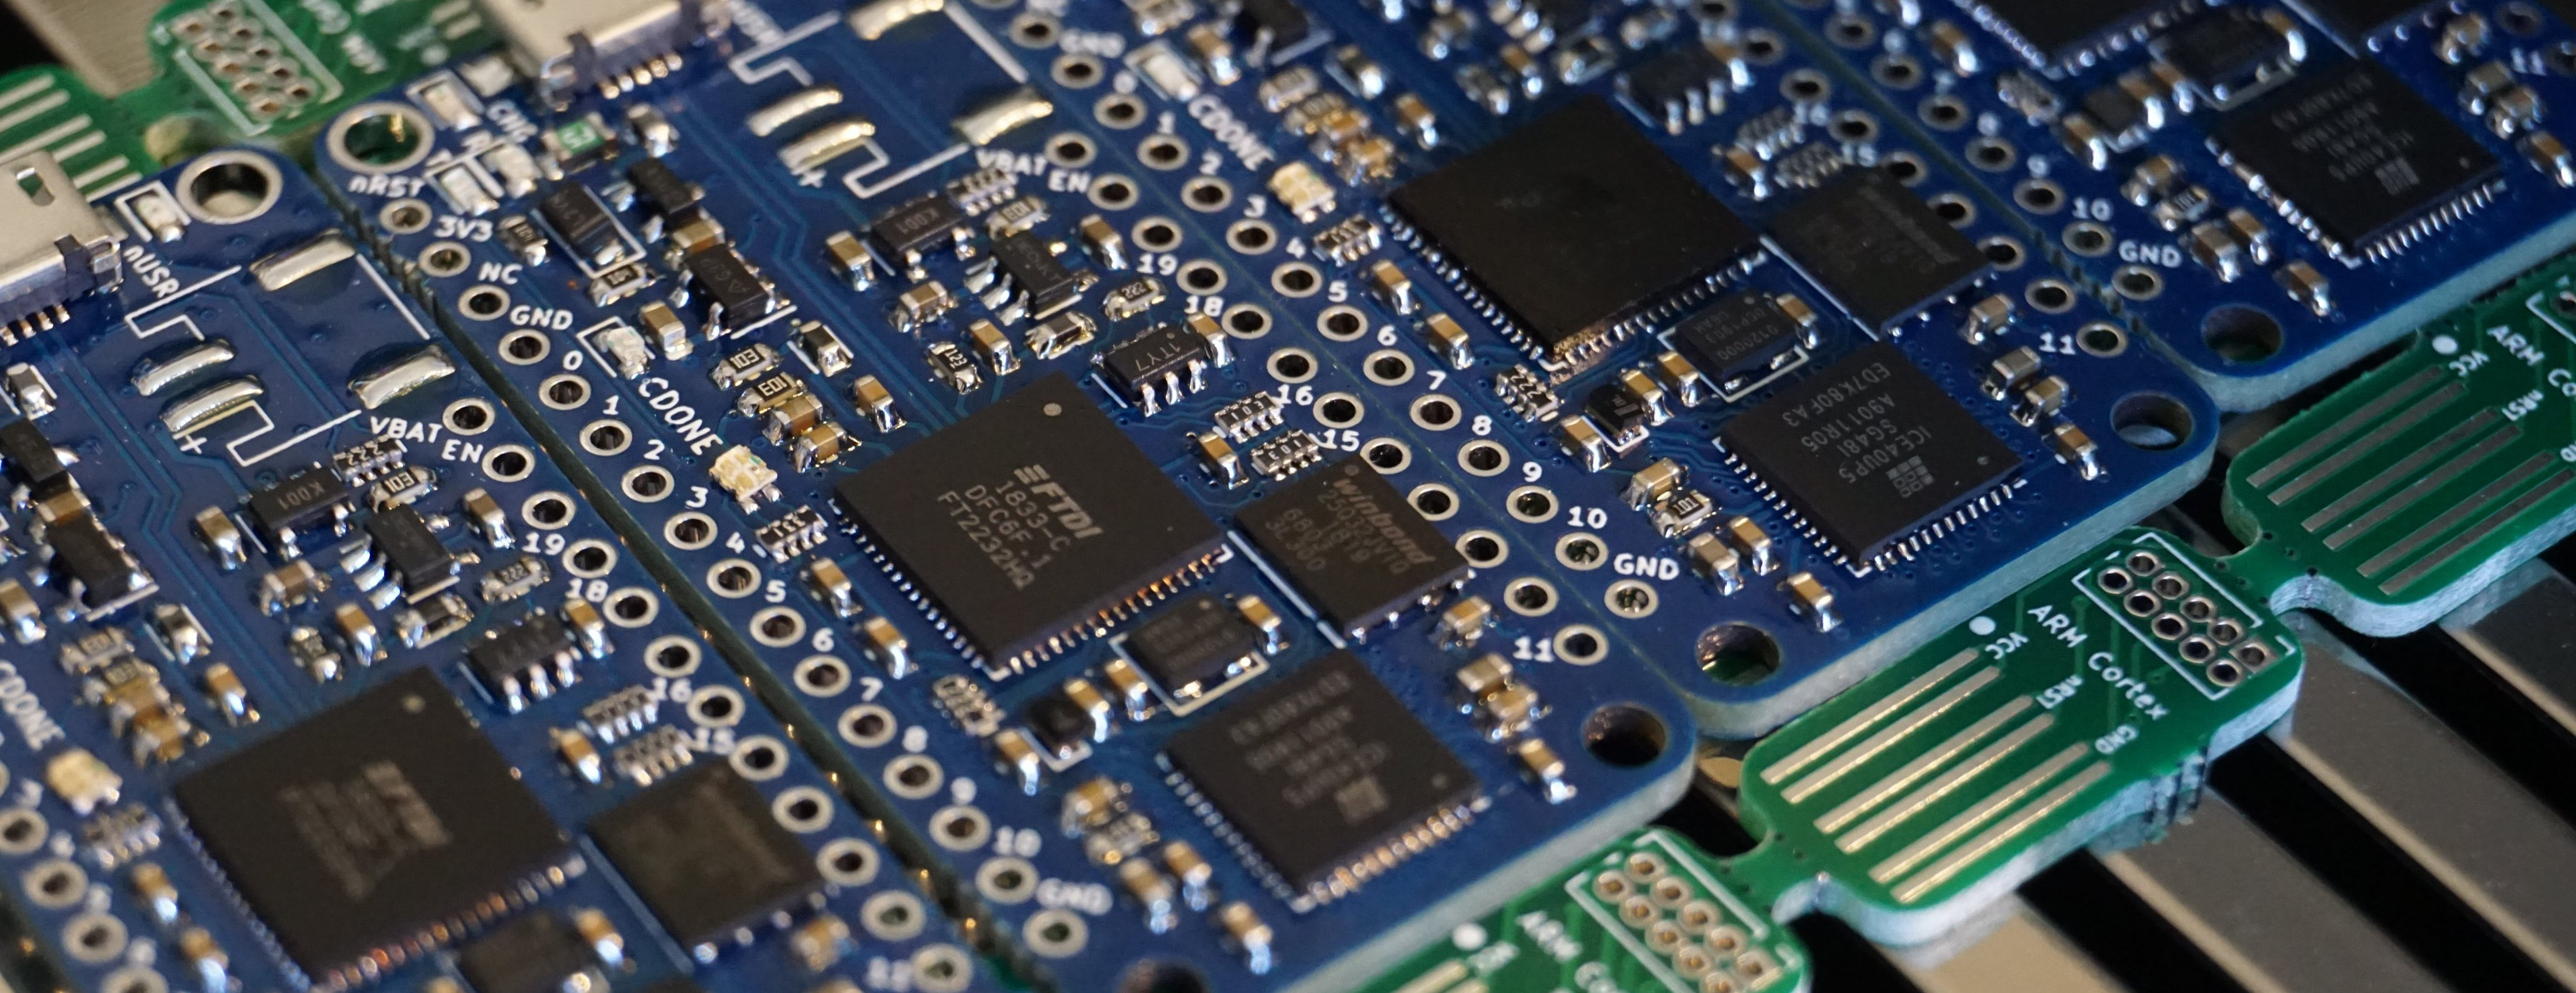
\includegraphics[width=0.8\linewidth]{images/ice40-reflow.jpeg}
\end{figure}
\end{frame}

\end{document}